\chapter{Simulationsumgebung}
\label{cha:simulationsumgebung}

Das Kapitel der Simulationsumgebung befasst sich mit den Eingabemöglichkeiten zur Anpassung der Simulationsparameter, sowie der konkreten Umsetzung der simulierten Welt, mit der Logik für die Notausgänge, der Personen, der Gefahrensituationen und dem Kommunikationsmodell.

Die Ausgangsbasis für die verwendeten Modelle und Protokolle stammen aus den erstellten Übungen zur Vorlesung Gensensornetze, sie wurden jedoch auf die Anforderungen der Hausarbeit adaptiert.

\section{Benutzerschnittstelle}
\label{sec:benutzerschnittstelle}


\section{Personen}
\label{sec:personen}

% Lifecycle
\subsection{Zustände}

% INIT
% INIT, DEAD
% INIT, RESCUED
% INIT, EVENT_DETECTED, DEAD
% INIT, EVENT_DETECTED, FLEEING, RESCUED
% INIT, EVENT_DETECTED, FLEEING, DEAD

\begin{figure}
\centering
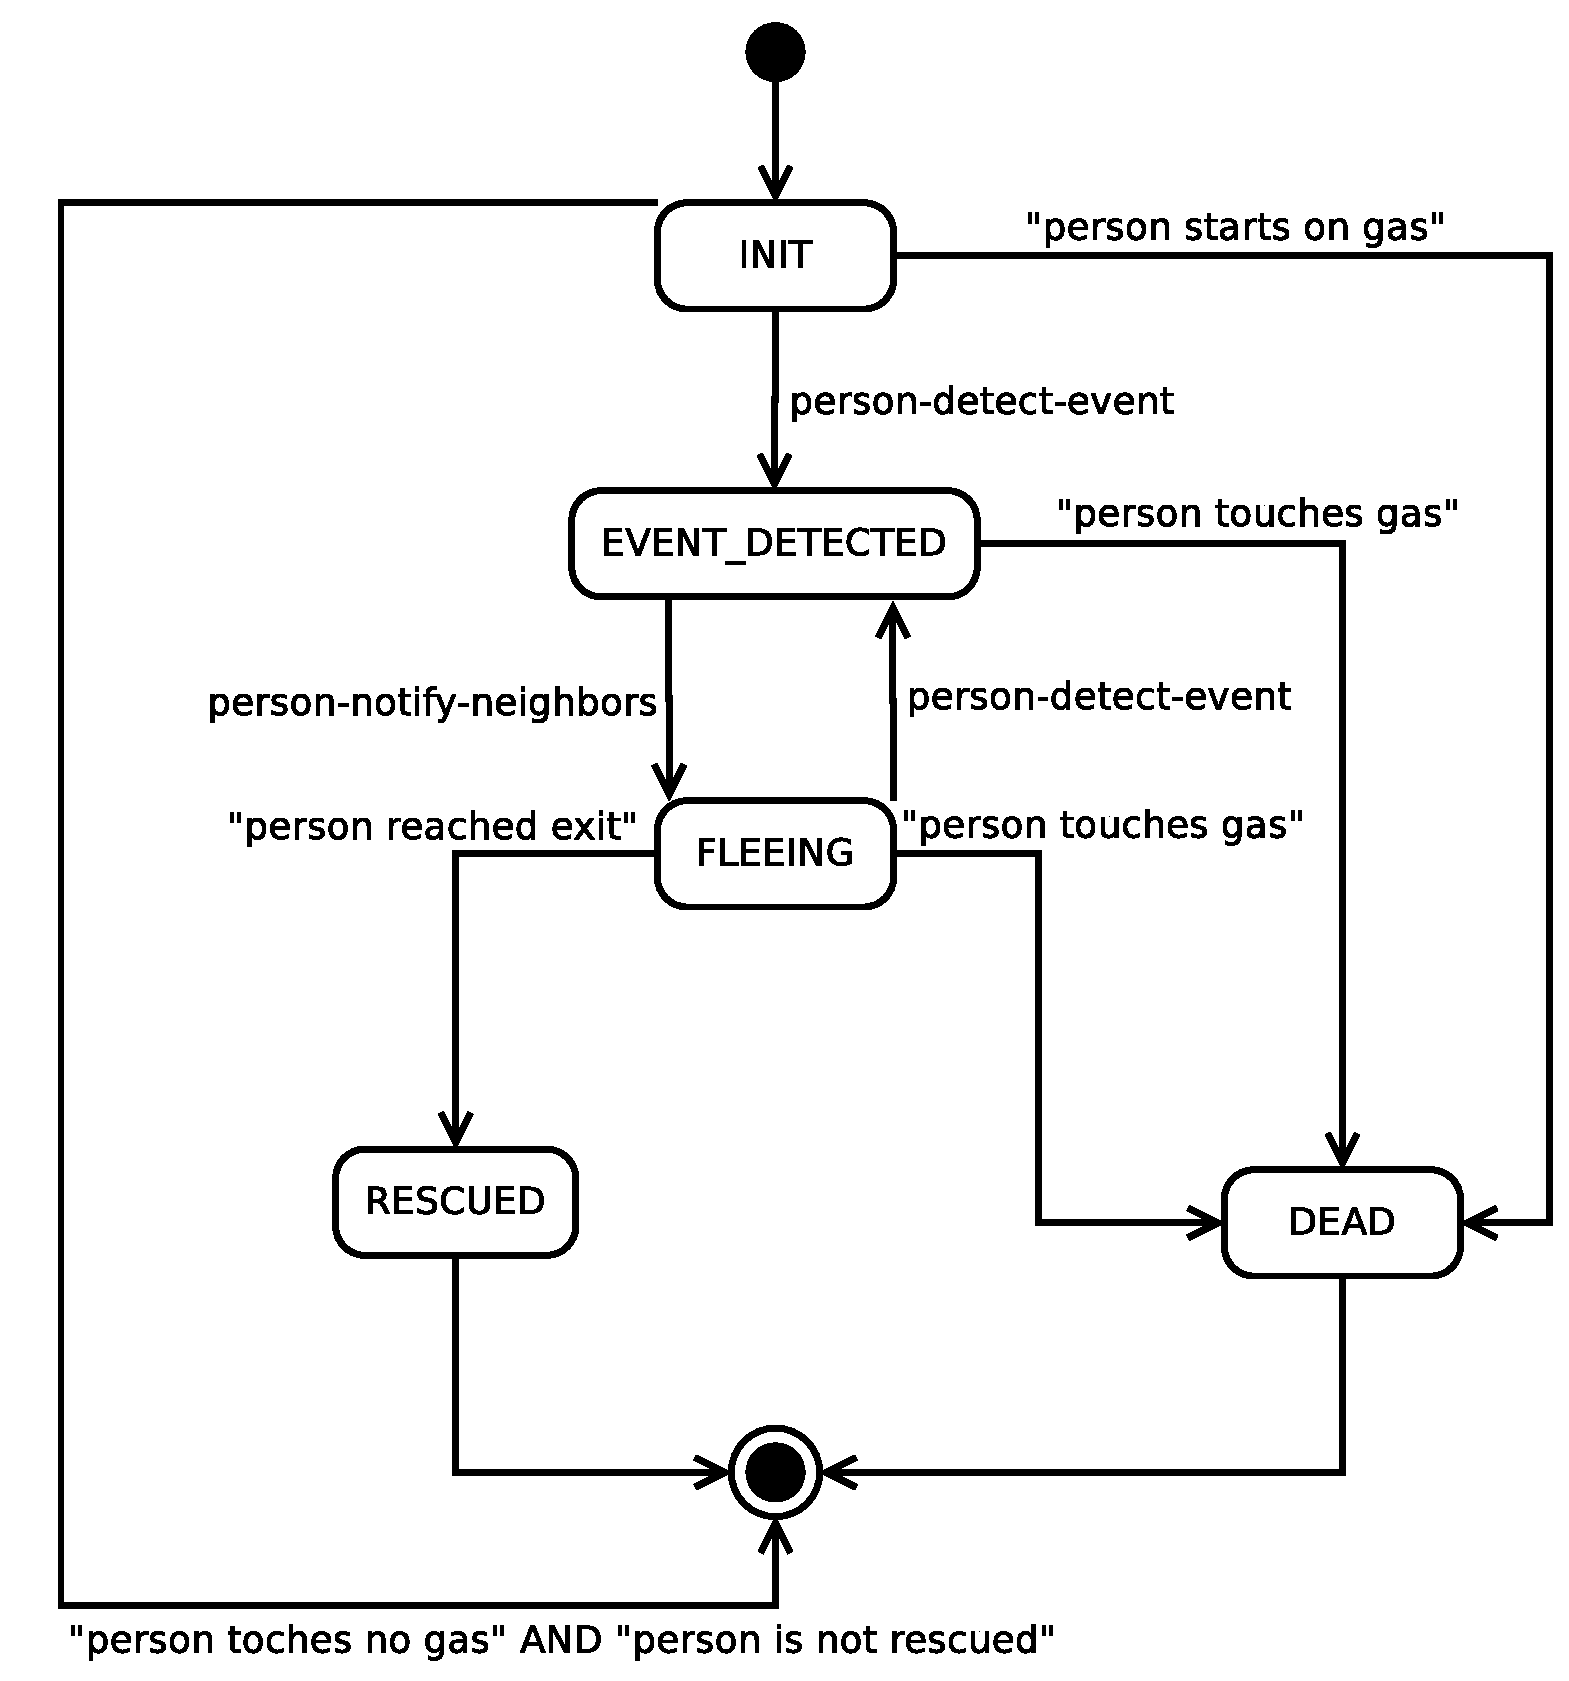
\includegraphics[height=0.6\textwidth]{simulationsumgebung/person.eps}
\caption{Zustandsdiagramm der Personen}
\label{fig:person}
\end{figure}

\subsection{Bewegungsmodell}
\label{sec:bewegungsmodell}
%Bewegungsmodell: Die Agenten sollen sich nach einem „Random Walk“ Modell bewegen. Agenten können Gefahren in ihrer Umgebung wahrnehmen und die Information an ihre nächs-ten Nachbarn weitergeben. Sobald ein Agent Informationen über eine Gefahrensituation hat, soll er sich auf dem kürzesten Weg zum nächsten Notausgang bewegen.  Hat ein Agent die Umgebung eines Notausgangs erreicht, soll er aus der Simulation genommen werden.

Dieser Abschnitt beschreibt zunächst das Bewegungsmodell der Personen ohne aktive Gefahrensituation.


\subsection{Kommunikationsmodell}
\label{sec:kommunikationsmodell}
%Kommunikationsmodell: Als Kommunikationsmodell können beliebige Modelle der Vorlesung implementiert werden. Dabei sollte insbesondere auf die dynamische Netzwerktopologie geach-tet werden. 



\section{Notausgänge}
\label{sec:notausgaenge}
%Notausgänge: Notausgänge sollen als statische Sensorknoten modelliert werden, die ihre Po-sition sowie Information zu ihrer Passierbarkeit im Netz verteilen. Die Positionen dieser sog. anchor nodes sollen zur Positionierung der mobilen Sensorknoten verwendet werden (Algorithmik). Während einer Simulation sollte der Ausfall einzelner Notausgänge simuliert werden.

%Lifecycle
\subsection{Zustände}

% INIT, NEGOTIABLE
% INIT, NEGOTIABLE, BLOCKED

\begin{figure}
\centering
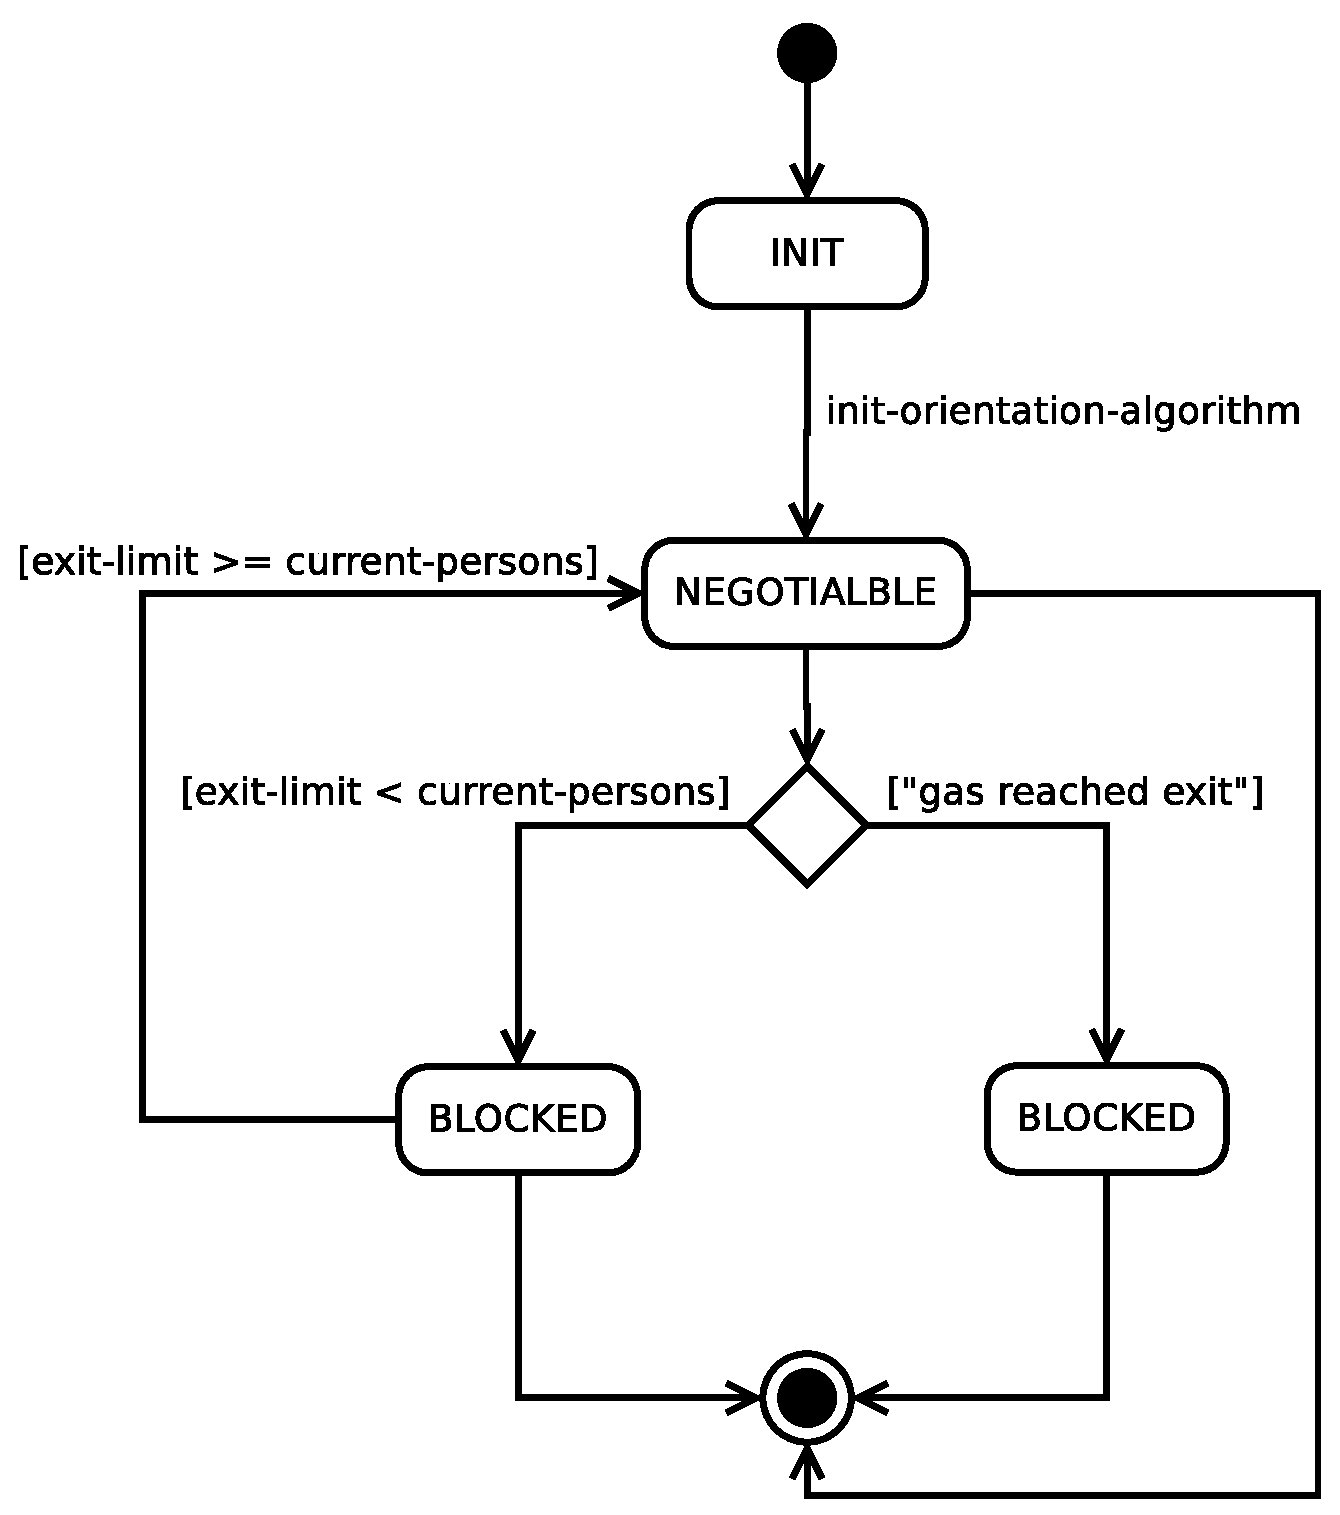
\includegraphics[height=0.6\textwidth]{simulationsumgebung/exit.eps}
\caption{Zustandsdiagramm der Notausgänge}
\label{fig:exit}
\end{figure}

\section{Gefahrensituationen}
\label{sec:gefahrensituationen}
%Gefahrenevents: Gefahrenevents erscheinen an zufälligen Orten im Grundriss. Ihr Erscheinen sollte zur vollständigen Evakuierung des Areals führen.

%Lifecyle
\subsection{Zustände}

% INIT, COUNTDOWN, GASSING, DONE

\begin{figure}
\centering
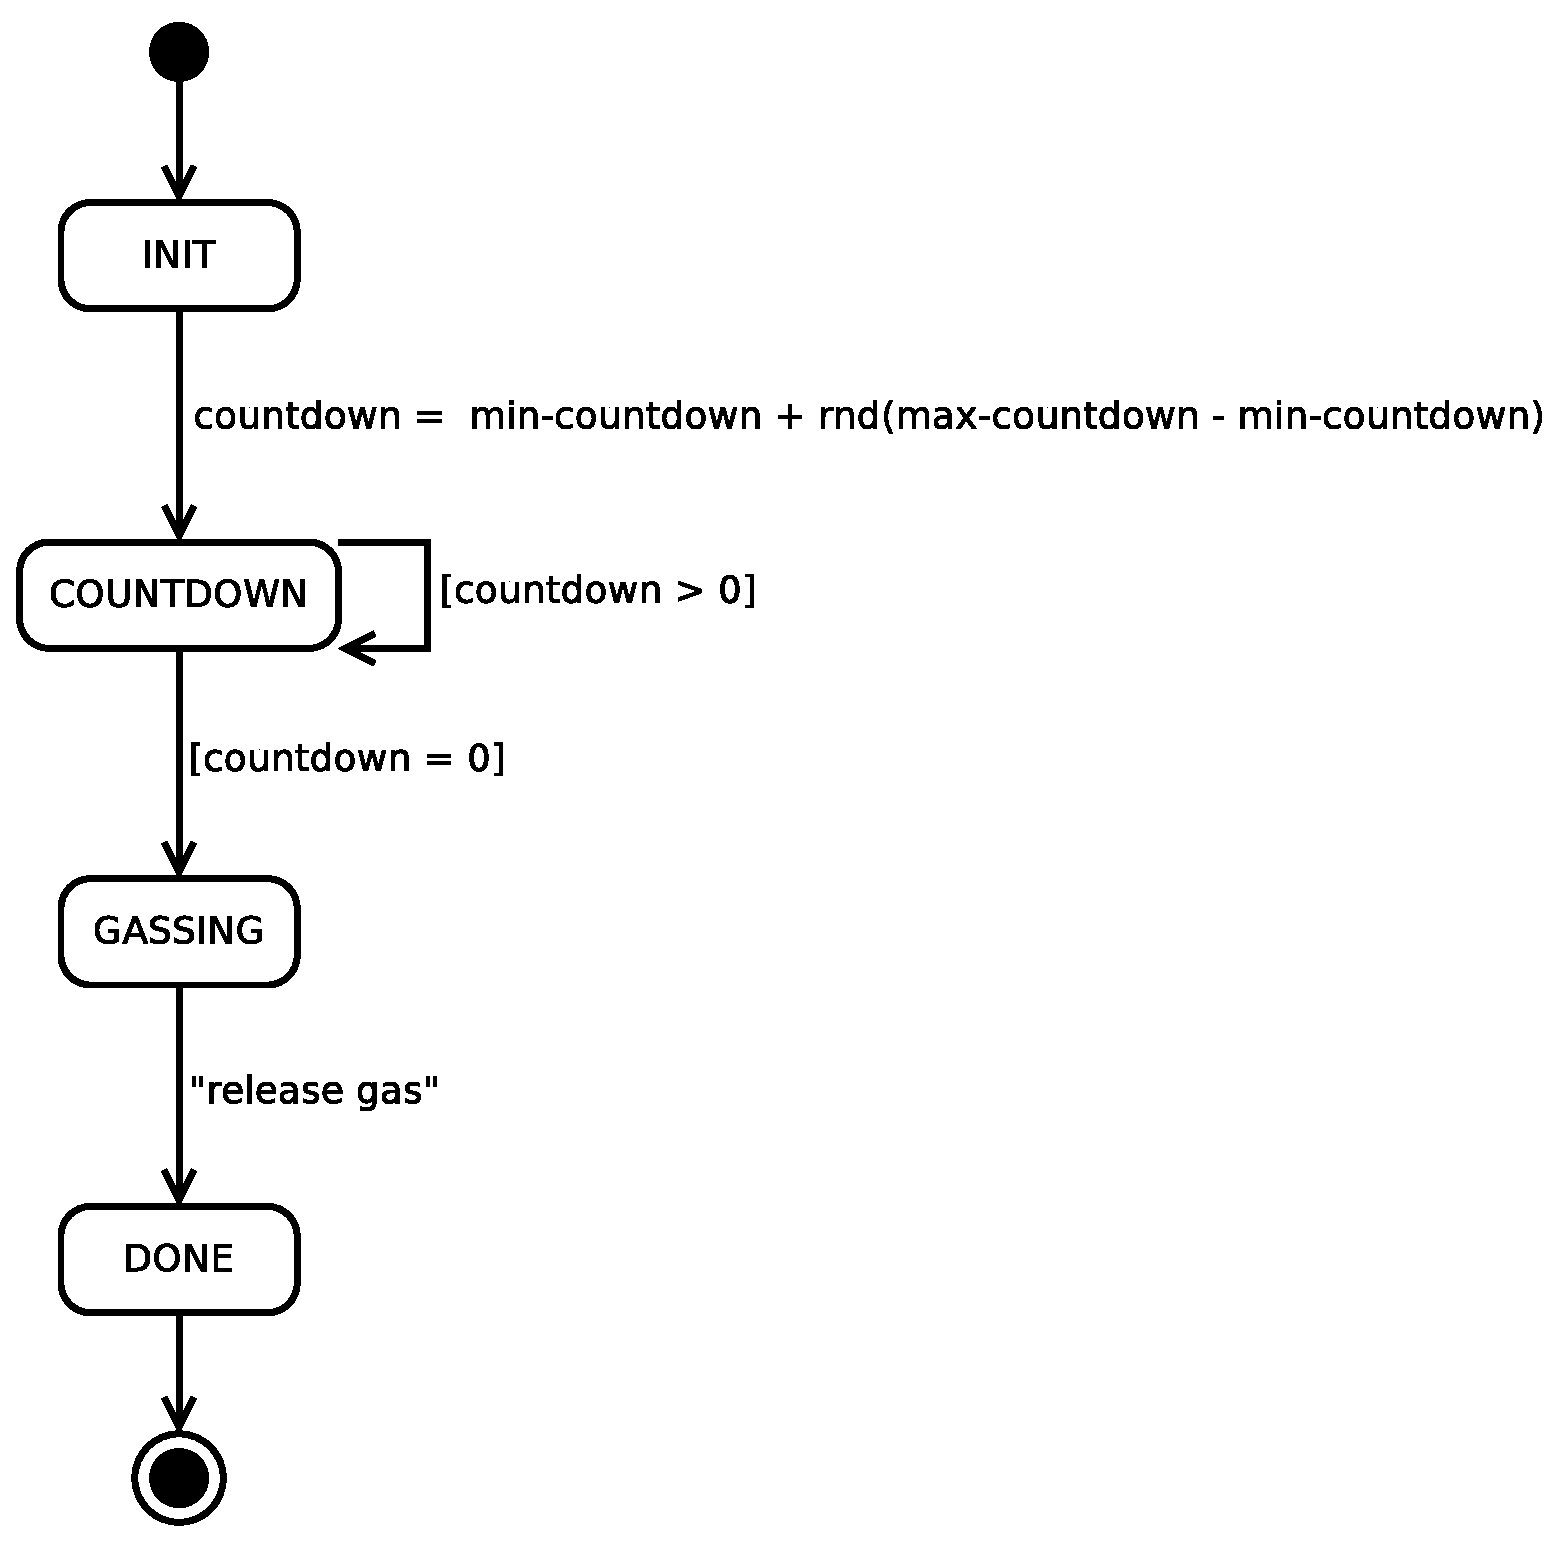
\includegraphics[height=0.6\textwidth]{simulationsumgebung/event.eps}
\caption{Zustandsdiagramm der Gefahrenevents}
\label{fig:event}
\end{figure}


\section{Patches}
\label{sec:patches}

%Lifecyle
\subsection{Implizite Zustände}

% NONE, WALL, SPREADING, IDLE, DONE, EVENT, EVENT-DONE

% Kategorie: Grundriss
% NONE
% WALL

% Kategorie: Zellulärer Automat
% NONE
% NONE, SPREADING, IDLE, DONE

% Kategorie: Gefahrensituation
% NONE, EVENT
% NONE, EVENT, EVENT_DONE
% DONE, EVENT
% DONE, EVENT, EVENT_DONE

\begin{figure}
\centering
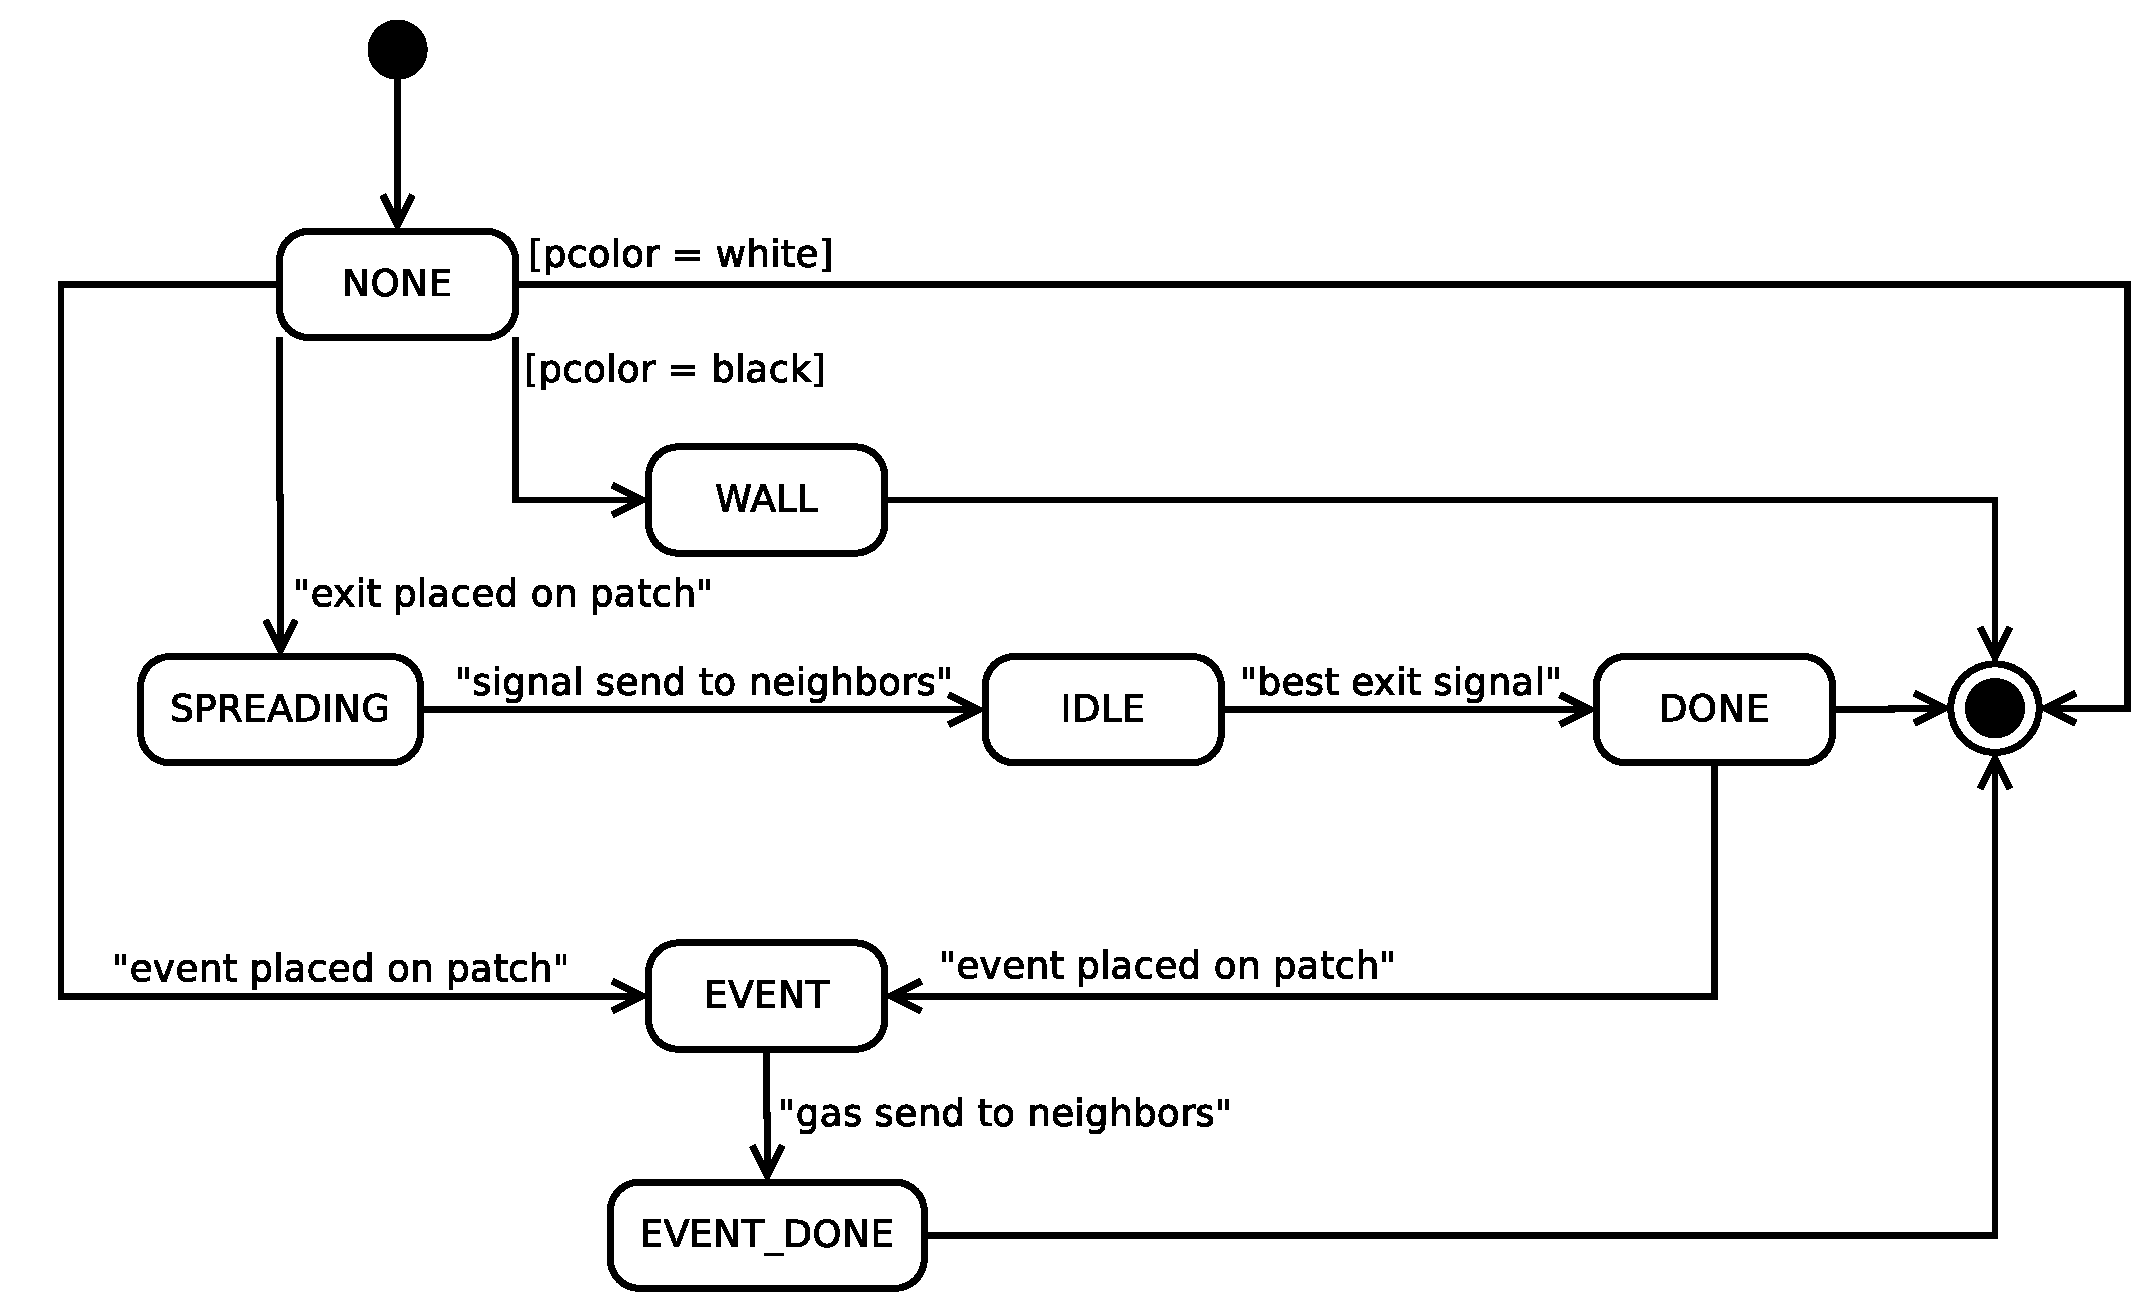
\includegraphics[height=0.6\textwidth]{simulationsumgebung/patch.eps}
\caption{Zustandsdiagramm der Patches}
\label{fig:patch}
\end{figure}

\section{Ressourcen der Simulationsumgebung}
\label{sec:ressourcen}

Die Simulationsumgebung wird über die Datei \verb|Evakuierung.nlogo| gestartet. Der Programmcode ist nach Funktion und \emph{Breed}-Klasse unterteilt.

\paragraph{Gefahrensituationen} 

\begin{verbatim}
event.nls
event-gassing.nls
\end{verbatim}

Die Quellcode-Datei \verb|event.nls| beinhaltet den Lebenszyklus der Gefahrenevents und deren Zustandsübergangsprotokoll. Mittels \verb|event-gassing.nls| wird die Ausbreitung des Giftgases implementiert, die größtenteils den Patch-Lebenszyklus manipuliert.

\paragraph{Lokalisierung}

\begin{verbatim}
locate.nls
\end{verbatim}

In dieser Datei wird der Algorithmus zur Lokalisierung aus dem Paper \cite{Jonathan.2004} implementiert.

\paragraph{Notausgänge}

\begin{verbatim}
exit.nls
exit-cellular-automaton.nls
exit-gsn.nls
\end{verbatim}

Die Quellcode-Datei \verb|event.nls| steuert den Setup und den Lebenszyklus der Notausgänge. Mittels \verb|exit-cellular-automaton.nls| wird der Orientierungsalgorithmus auf Basis des zellulären Automats realisiert. Letztlich definiert die Datei \verb|exit-gsn.nls| das Kommunikationsmodell zur Übermittlung der Statusinformationen.

\paragraph{Personen}

\begin{verbatim}
person.nls
person-gsn.nls
person-linking.nls
\end{verbatim}

\verb|person.nls| regelt den Setup der Personen und deren Lebenszyklus. \verb|person-gsn.nls| umfasst den Quellcode für die Kommunikation zwischen Personen und mit der Datei \verb|person-linking.nls| wird der Graph zwischen Personen erstellt.

\paragraph{Simulationswelt}

\begin{verbatim}
patch.nls
\end{verbatim}

Hier wird der Quellcode für den Lebenszyklus der \emph{Patches} definiert.